\documentclass[a4paper,english]{article}
\usepackage{graphicx}
\usepackage[T1]{fontenc}
\usepackage[utf8]{inputenc}
\usepackage{babel}
\usepackage{hyperref}
\usepackage{upgreek} %proper greek letters
\usepackage{fullpage}
\usepackage{lineno}
\usepackage{amsmath} % typesetting math
\usepackage{amssymb}
\usepackage{booktabs} % nice tables
\usepackage[round,sort&compress]{natbib}
\usepackage{pdfpages} %include external pdfs
\usepackage{enumitem} %for noitemsep in lists
\usepackage{csquotes} %for noitemsep in lists
\usepackage{subfig}
\renewcommand{\arraystretch}{1.2} % space in tables
\usepackage{authblk}
% \usepackage[toc,page]{appendix} %for appendix titles
% \usepackage[titletoc,title]{appendix} %for appendix titles
\usepackage[colorinlistoftodos,prependcaption,textsize=tiny]{todonotes} %todo note in margin

\begin{document}

\title{Comparison of Multi-Parallel Slit and Knife-Edge Slit Prompt Gamma Cameras in the context of hadrontherapy verification}

\author[1,2]{Brent F. B. Huisman}
\author[2]{É. Testa}
\author[1]{D. Sarrut}
\affil[1]{~CREATIS, Université de Lyon; CNRS UMR5220; INSERM U1206; INSA-Lyon; Université Lyon 1; Centre Léon Bérard, Lyon, France}
\affil[2]{~IPNL, Université de Lyon; CNRS/IN2P3 UMR5822; Université Lyon 1 Lyon, France}
\affil[ ]{~E-mail: brent.huisman@cern.ch}

\maketitle

\begin{abstract}

\emph{Purpose:} 

\emph{Materials and Methods:} 

\emph{Results:} 

\emph{Conclusion:} 

\end{abstract}

\tableofcontents

\newpage

%%%%%%%%%%%%%%%%%%%%%%%%%%%%%%%%%%%%%%%%%%%%%%%%%%%%%%%%%%%%%%%%%%%%%%%%%%%%%%%%
\section{Introduction}

\paragraph{State of the art} At the moment, two papers have proposed a comparison of MPS-KES cameras:
\begin{itemize}
	\item Smeets 2016 Fontiers in Oncology: experimental comparison with a non-optimized CLaRyS MPS camera (some technical constraints prevented the authors to use the \enquote{optimal CLaRyS design})
    \item Lin 2017 Radiation Physics and Chemistry : MC comparison with the MPS Korean design whose optimization procedure is actually questionable
\end{itemize}
In overall, the camera configurations present many parameters, namely geometrical parameters and event selections (especially energy deposition selection). Therefore, in principle, some theoretical expectations are required to set relevant parameters and to allow for a fair comparison of the two types of collimators. Although the aforementioned studies may give the impression to provide a fair comparison (use of the same absorbers, same beam-collimator and collimator-absorber distance in the case of Lin 2017), they do not provide a thorough justification of their sets of parameters. Surprisingly, some parameters are even not the same between the two camera types. While it can be understood in Smeets 2016 due to experimental constraints, it is more questionable Lin 2017 (different energy deposition selection).

\paragraph{Objectives}
The objectives of the present paper are the following:

\begin{itemize}
  \item Estimate the MPS and KES detection efficiencies and spatial resolution from geometrical considerations
  \begin{itemize}
    \item Draw some conclusions about the intrinsic features of MPS and KES collimators:  
    \item Estimate various MPS and KES performances 
    \begin{itemize}
    	\item In Smeets 2016 and Lin 2017: the KES/MPS detection efficiency ratio is 1.6 for Smeets 2016 and 5.3 for Lin 2017 (assuming the use of the same energy window) $\Rightarrow$ these comparisons were unfair\dots    
        \item "Official" MPS and KES prototypes with identical absorbers 
    \end{itemize}    
  \end{itemize}
  \item MC simulation: geometrical considerations verification and prototype direct comparison
\end{itemize}  

%%%%%%%%%%%%%%%%%%%%%%%%%%%%%%%%%%%%%%%%%%%%%%%%%%%%%%%%%%%%%%%%%%

\section{Materials and Methods}

%%%%%%%%%%%%%%%%%%%%%%%%%%%%%%%%%%%%%%%%%%%%%%%%%%%%%%%%%%%%%%%%%%%%%%%%%%%%%%%%

\subsection{Features of PG profiles}

Figure~\ref{ProfileParameters} defines the 3 parameters of a typical PG profile measured with a collimated camera in the falloff region and in the case of a homogeneous target irradiation.

\begin{figure}[htp]
  \centering
  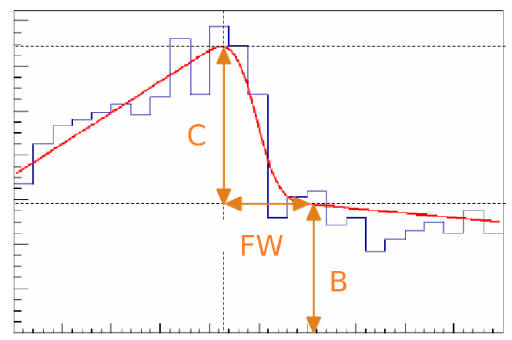
\includegraphics[width=.45\textwidth]{ProfileParameters}
  \caption{\label{ProfileParameters} PG profile parameters.}
\end{figure} 

The 3 parameters are the following:
\begin{itemize}
  \item the contrat $C$ corresponding to the falloff amplitude,
  \item the background level $B$,
  \item and the falloff $FW$ width related to the camera spatial resolution (Note that the PG emission profile has an intrinsic width of a few millimiters. In practice the width of PG emission profiles measured by the collimated camera prototypes is dominated by the camera resolution of the order of 20 mm).
\end{itemize}

As expected, these 3 parameters have very different impacts on the falloff retrieval precision ($FRP$). As mentioned in [Roellinghoff MPB 2014], $FRP$ is mainly determined by the contrast-to-noise ratio of the profile. The detailed study of the influence of $C$, $B$ et $FW$ on $FRP$ has shnown that [Roellinghoff PhD thesis 2014]:
\begin{itemize}
 \item $FRP\propto \frac{\sqrt{B}}{C}$
 \item The influence of $FW$ is negligible
\end{itemize}

As a consequence, the optimization of the collimated cameras is actually a compromise between $FRP$ and spatial resolution $FW$. In principle, collimator slits have to be as large as possible to increase detection efficiency and minimize $FRP$. However, a \enquote{reasonable} spatial resolution has obviously to be defined and it has been set in the range of $\sim1$ to 2 cm depending on the collimator types. Morevover, this spatial resolution can play a major role in clinical conditions since the beam might cross highly heretrogeneous regions. More specifically, Priegnitz et al. have shown that the KES prototype is not able to detect the filling of a cavity located 5~mm upstream to the Bragg peak position [Priegnitz PMB 2015].


\subsection{Geometrical considerations}



\begin{table}
\centering
\begin{tabular}{lllll}
	\midrule
	                            & MPS & MPS calc. & KES & KES calc. \\
	\midrule
	Effective slit width ($s_e$)& $s$                              & 5.4 mm
	 & $s + \frac{ln(2)}{\mu~tan(\alpha)}$                         & 6 mm (TODO add transparency) \\
 	Det. unit FOV               & $s(1+\frac{d_1}{D})$             & 14.52 mm
 	 & $s_e(1+\frac{d_1}{d_2})$                                    & 13.5 mm\\
 	Lin. collection efficiency  & $\frac{H s}{ 4 \pi L D } (1-f) $ & $4.18 \cdot 10^5$
 	 & $\frac{H s}{ 4 \pi L d_2 } (1 + x^2/d^2_2)^{-3/2} $         & $6.67 \cdot 10^5$ \\
 	Effective thickness ($T_e$) & $D_f$                            & 58.5 mm
 	 & $T$                                                         & 40 mm\\
	\midrule
\end{tabular}
\caption{MPS and KES detection efficiencies and spatial resolution from geometrical considerations. The parameters of the cameras are defined in figure~\ref{GeomSchemes}.}
\label{GeomFormulas}
\end{table}

%\begin{figure}[htp]
%    \centering
%    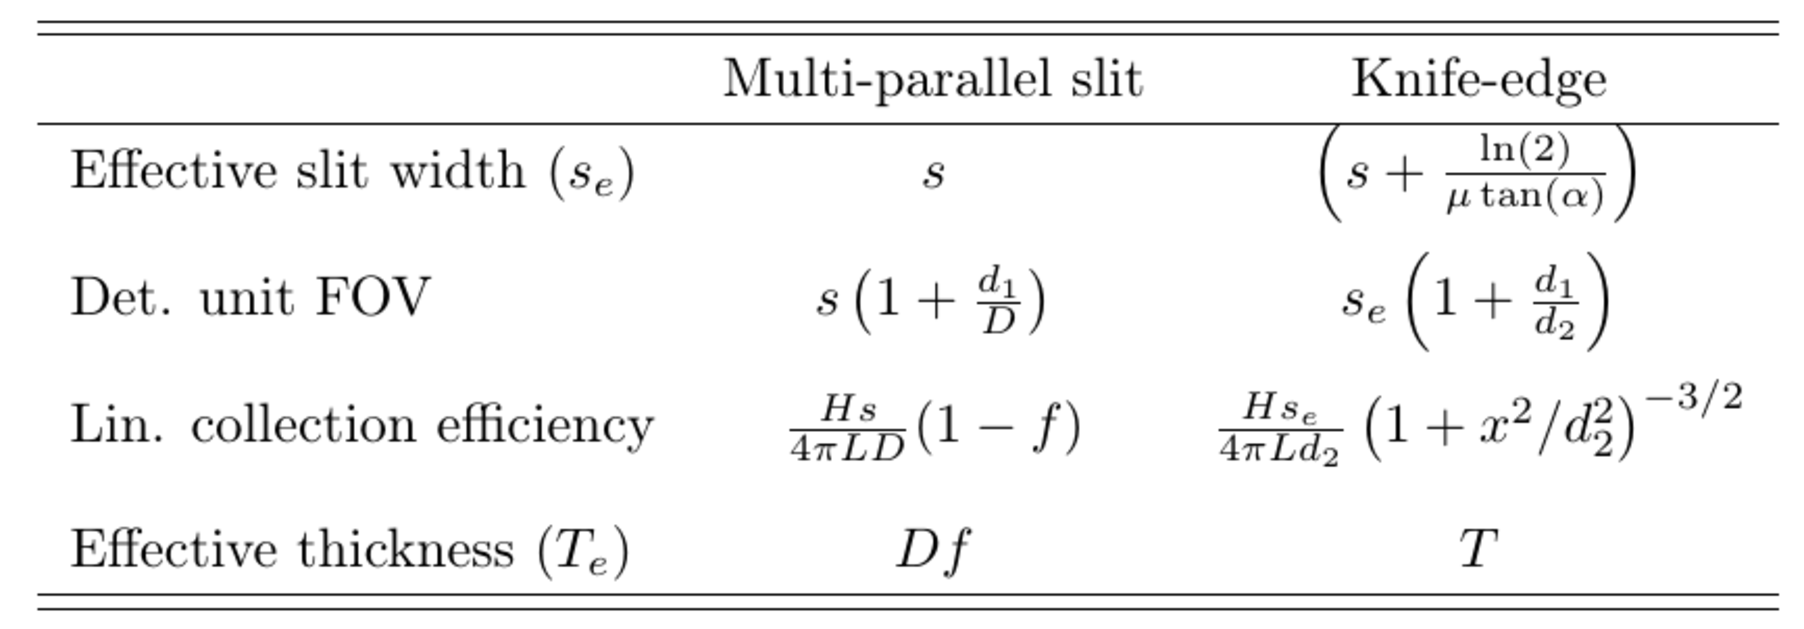
\includegraphics[width=.85\textwidth]{FormuleMPS-KES}
%    \caption{MPS and KES detection efficiencies and spatial resolution from geometrical considerations. The parameters of the cameras are defined in figure~\ref{GeomSchemes}.  }
%  \end{figure}



\begin{itemize}
  \item Rationale: geometrical considerations should provide good predictions of collimated camera performances while providing a good understanding of the intrinsic features of the 2 types of collimators. 
  \item Estimate the MPS and KES performances in Smeets 2016 and Lin 2017: the KES/MPS detection efficiency ratio is 1.6 for Smeets 2016 and 5.3 for Lin 2017 (assuming the use of the same energy window) $\Rightarrow$ these comparisons were unfair\dots    
\end{itemize}

\subsubsection{Parameters}

\begin{itemize}
  \item Geometrical parameters (Figure~\ref{GeomSchemes})
  \item Energy and TOF selections
\end{itemize}

\begin{figure}[htp]
    \centering
    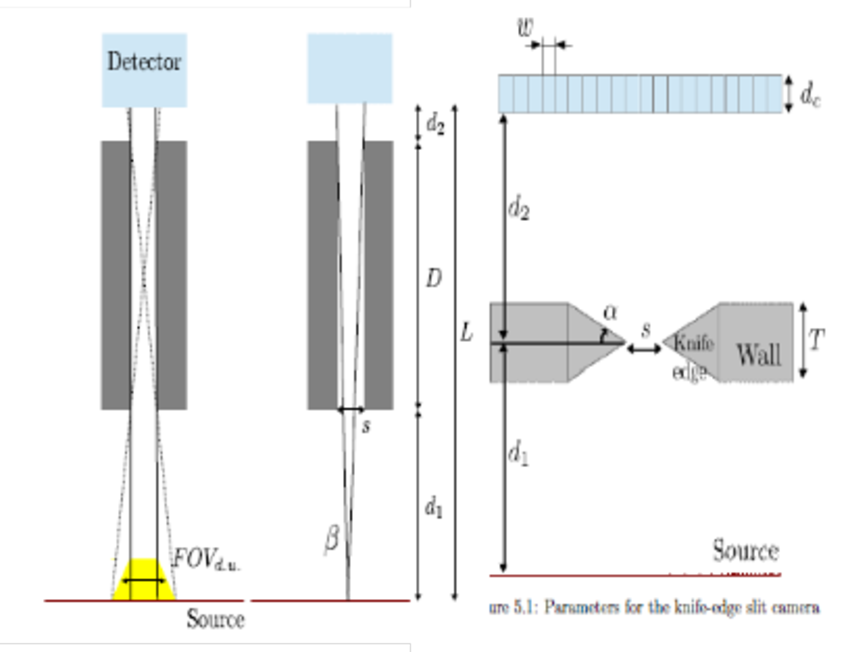
\includegraphics[width=.45\textwidth]{SchemeMPS-KES}
    \caption{\label{GeomSchemes}Schemes of MPS and KES cameras.}
\end{figure}          

\subsubsection{Definitions and figures of merit}



\paragraph{Definitions}

\begin{itemize}
  \item Detector unit field of view: This is the part of the source that can be “seen” through a single camera unit: a single slit for the MPS (naturally associated to a single detector unit) and a single detector unit for KES. The probability of a photon emitted at a given point along a linear source (perpendicular to the slit plane) to reach this detector unit can be described as a trapezoid: the part that can be seen from every points on the detector unit and the penumbra.
  \item Collection efficiency: The probability of a photon emitted at a point facing a slit (in the middle part of the trapezoid) to reach the detector is described by the solid angle that the point sees of the detector.
  \item Linear collection efficiency: collection efficiency divided by the pitch that corresponds to the collection efficiency of the camera per unit of length
  \item Effective Slit Opening (especially for KES): At the particle energies that occur in prompt-gamma imaging, a non-negligible amount of particles will cross the collimator slit edges. This effect can be approximated by introducing an effective slit opening that can be used in the evaluation of the field of view and the efficiency in place of the geometrical slit opening. 
  \item Spatial resolution: PSF width. In the context of PG detection, the gamma source can be considered at first order as a linear source. Hence one can estimate the spatial resolution of the collimated camera from the derivative of the PG profile that has a gaussian-like shape. The width of the derivative can be defined as the spatial resolution of the collimated cameras in the context of PG detection.
\end{itemize}

\begin{figure}[htp]
    \centering
    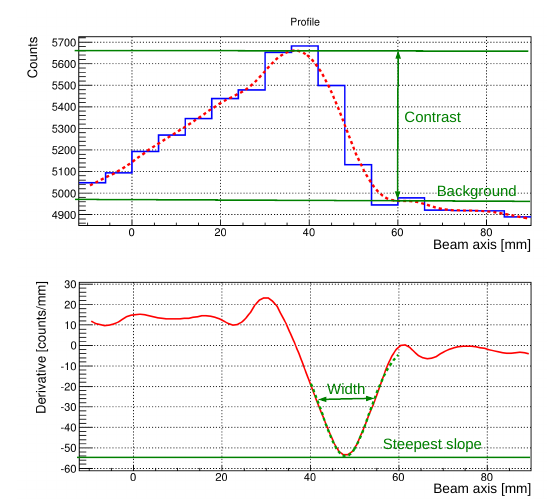
\includegraphics[width=.45\textwidth]{PGprofile_FW}
    \caption{\label{PGprofile_FW}Example of PG profile falloff width (FW) estimate with the first derivative of the PG profile (Figure 4.15 of Frauke's manuscript).}
\end{figure}          



\subsection{Monte Carlo simulations}

\begin{itemize}
  \item Geometrical considerations verification: Fair comparison of the two types of collimators with MC simulations. What does it mean? 
  \begin{itemize}
    \item Use of same absorbers (the LYSO absorber of the KES prototype that we can consider as the reference), the same energy selection which was not the case in Lin 2017 and the same TOF selection (no TOF)
    \item Then a discussion of the results in the light of the geometrical considerations
    \item Note: the KES background level can be obtained from Figure 18 in Perali 2014. Regarding the MPS background level I propose to use the same level as the one of KES for the following reasons: i) the background level in the MPS camera is derived in Pinto 2014 from measurements with large detectors by assuming that the background is proportional to the detector volume. If we apply the same approach, it is reasonable to use the same background levels since we use the same absorbers for MPS and KES. One can argue that the MPS and KES collimators are different. It is true and it is difficult to say whether the larger amount of material in the CLaRyS MPS collimator leads to a larger background with more neutron-induced gammas or a lower background due to a larger attenuation of these gammas\dots At first order the background levels should be similar and a first order estimate is sufficient for a paper that mainly aims at comparing the signal detection of the two cameras.
  \end{itemize}    
  \item Simulations of the two prototypes as they are published (results of the submitted paper with the \enquote{regular} cylindrical PMMA target of 15 cm diameter and 20 cm lenght). 
  \begin{itemize}
    \item $\Rightarrow$ Comparison of the two prototypes
    \item Identification of the impact of energy (>1 MeV vs 3-6 MeV selection for KES) and TOF selection (for MPS) although the latter has been already shown in Roellinghoff PMB 2014 with a large detector placed behind a single slit collimator
    \item Note that the absobers have different thicknesses
  \end{itemize}     
\end{itemize}

\subsubsection{Simulation tool}

Imaging paradigms such as PG detection are evaluated against experiments, and often also with Monte Carlo (MC) simulations~\citep{Moteabbed2011,Gueth2013,Robert2013,Golnik2014a,Janssen2014}. For rarely occurring processes such as PG simulation, convergence to the model of the truth to within acceptable statistical error can be slow. This paper presents an \emph{in silico} study of the feasibility of the clinical relevance of PG FOP estimation using collimated cameras, and uses the vpgTLE variance reduction method described in \cite{Huisman2016}. vpgTLE is a two stage process, where firstly a PG yield distribution image is estimated, which in the second stage is used as a PG source with which detectors can be investigated. Gate 7.2~\citep{Sarrut2014} with Geant 4.10.02 and the QGSP\_BIC\_HP\_EMY physics list, commonly used for PG studies, are used in this analysis. Thanks to vpgTLE, simulations for about $10^9$ protons (about $6\times10^8$ photons) took 1-2 hours on a single core of an Intel(R) Core(TM) i7-3740QM.

%%%%%%%%%%%%%%%%%%%%%%%%%%%%%%%%%%%%%%%%%%%%%%%%%%%%%%%%%%%%%%%%%%%%%%%%%%%%%%%%
\subsubsection{PG camera modeling}\label{sec:camera}


Two PG detectors tailored to FOP verification (illustrated in fig.~\ref{fig:detectors}) were chosen:
\begin{itemize}[noitemsep]
\item the CLaRyS multi-parallel-slit (MPS) camera, Case 1 \citep{Pinto2014a}
\item[] This camera intends to measure the whole PG profile to control ion-ranges in the patient with a field of view (FoV) of 300 mm. It makes use of ToF selection to reduce the neutron background. In the optimization carried out by \cite{Pinto2014a}, parameters such as collimator pitch, axis-to-collimator and axis-to-detector were varied, and their impacts evaluated in terms of fall-off retrieval precision (FRP) and spatial resolution (sharpness of the fall-off region). Here, configuration 1 (with relaxed constraints on spatial resolution) was chosen for its optimal FRP performance. As was done by \cite{Pinto2014a}, the camera lengths (collimator and scintillator volume) are chosen \emph{up to} 300 mm, such that the length is an integer multiple of the pitch size, with for the collimator a collimator-leaf-width extra, to ensure each pixel has a leaf on both sides. With the 8 mm pitch and 2.6 mm collimator-leafs, this results in a scintillator volume of length 296 mm and collimator length 298.6 mm.
\item the IBA knife-edge (KES) camera \citep{Perali2014,Sterpin2015}
\item[] The purpose of this camera consists of verifying the BP position with a FoV of 100 mm. \cite{Richter2016} provides the first clinically obtained results. At this time, no other camera has been subjected to clinical tests, which is why we consider this prototype a benchmark.
\end{itemize}

\begin{figure}[htp]
  \centering
  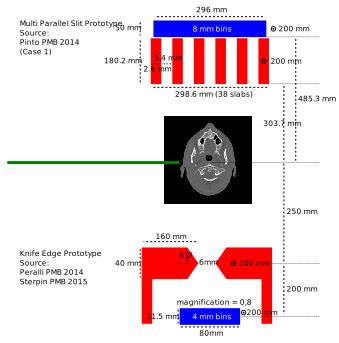
\includegraphics[width=0.9\linewidth]{detectors}
  \caption{Schematic presentation of the two PG cameras considered in this study. The green arrow represents the proton beam. In red the collimation elements and in blue detection elements. The dimensions were taken from \cite{Pinto2014a} and \cite{Perali2014,Sterpin2015}. Note that the two cameras have an identical detector height ($\odot$ symbol), the two cameras were positioned at an identical location above the head during all simulations, and that here they are not drawn to scale.}
  \label{fig:detectors}
\end{figure}

Regarding background ToF selection, for the IBA C230 accelerator with a period of 10 ns, \cite{Pinto2014a} chose a window of 4 ns around the PG maximum, based on experimental ToF spectra. This means that about 60\% of the noise could be removed. For the KES prototype ToF is not used, leading to a higher background, as is evident when one compares the backgrounds as published in the two publications. A second difference is the energy selection window. The IBA group employ a 3-6 MeV window, whereas the CLaRyS collaboration produced their optimization with a 1-8 MeV window. We will compare each camera with their published properties, that is to say: a 1-8 MeV window and ToF for MPS and a 3-6 MeV window without ToF for KES.

Both PG camera prototypes have different photodetectors and different detector electronics. In this study, these differences are not implemented. Instead, the method as described in \cite{Gueth2013} was used to obtain the interaction point of an impinging photon. If the integrated energy deposited in a crystal lies in the acceptable energy and ToF window, the event is recorded. The position of the event in the crystal is considered as the energy weighed barycenter of all interactions in the crystal, plus a random value taken from a 5mm FWHM Gaussian to simulate the electronics and the detector resolution.

\paragraph{Fair Comparison}

Since we are using a simulation for the validation of the theoretical expressions in table~\ref{GeomFormulas}, for the fairest comparison possible, we can equalize certain aspects which might cause one camera or the other to give favorable impression. In principle this comparison is not about absorption materials, acquisition electronics or PG selections, but PG collimator characteristics. So, for the validation of the expressions in table~\ref{GeomFormulas} and comparison on LCE, SR and FRP we set the absorber material of the MPS to that of the KES: LYSO. The energy and ToF selection windows are kept identical for both cameras, and are varied in order to study their impact on the figures of merit.

%%%%%%%%%%%%%%%%%%%%%%%%%%%%%%%%%%%%%%%%%%%%%%%%%%%%%%%%%%%%%%%%%%%%%%%%%%%%%%%%
\subsubsection{Background estimation}

Background estimation in PG simulation is a difficult and largely unsolved issue \citep{Huisman2016,Sterpin2015,Pinto2014a,Perali2014}. Simulations would ideally include beam nozzle and whole room modeling, but these are habitually omitted. ToF selection techniques can improve the signal-to-noise ratio (SNR) \citep{Testa2008,Roellinghoff2014a}, but then depend on the proper simulation of the beam accelerator time structure. As noted in \cite{Huisman2016}, no validation for background in PG simulations has been performed at this time. In this study, the stable time structure of current generation cyclotrons was assumed, in which the neutron background is largely constant. Estimates of background counts in the detector are taken from \cite{Pinto2014a,Perali2014}, which are both based on measured data:

\begin{itemize}[noitemsep]
\item MPS: \cite{Pinto2014a} fig.~9: $1 \cdot 10^{3} \pm 1 \cdot 10^{2}$ per $4\cdot10^9$ primary protons per 8 mm bin
\item[] Converted to per primary proton: $2.5 \cdot 10^{-7} \pm 0.25 \cdot 10^{-7}$
\item KES: \cite{Perali2014} fig.~11: $5 \cdot 10^{-7} \pm 0.5 \cdot 10^{-7}$ per primary proton per 4 mm bin
\end{itemize}

Per unit of bin length, the background yield of the MPS with ToF is therefore 4 times as low as the background seen with the KES. In the context of the fair comparison, for the KES camera the background with ToF can be obtained by multiplying the background with the same $\frac{4 ns}{10 ns} = 0.4$ fraction as with the MPS.


%%%%%%%%%%%%%%%%%%%%%%%%%%%%%%%%%%%%%%%%%%%%%%%%%%%%%%%%%%%%%%%%%%%%%%%%%%%%%%%%
\subsubsection{Fall-off position estimation procedure}

From a clinical perspective, the range estimate could be more interesting than FOP, because it can distinguish simple offset errors from patient morphological change. While the MPS camera was conceived for whole range PG profile detection, the KES camera FoV was chosen for BP region PG detection only. To make the comparison fair, only the FOP could be considered. Multiple approaches to extracting a FOP from the line profile have been proposed \citep{Smeets2012,Gueth2013,Roellinghoff2014a,Janssen2014,Sterpin2015}. In preparatory work, a number of the proposed procedures were investigated. Significant sensitivity to free parameters on the final FOP estimates were seen. In summary, the FOP estimate depends greatly on the procedure, and often on having yields uncommon on the spot-level in clinical TPs, and also on an absence of unavoidable inhomogeneities.

Therefore the fitting method was not chosen as a topic for study in this paper. Instead, a simple method that works on most the data available to the authors was used: first a smoothed and interpolated spline function is fitted against the detected PG data points, after which a baseline and (distal) peak position are determined. The intersection of the spline with the half-height of the peak above the baseline is then taken as the FOP. A more detailed description of the procedure may be found in appendix~\ref{sec:fopproc}.

%%%%%%%%%%%%%%%%%%%%%%%%%%%%%%%%%%%%%%%%%%%%%%%%%%%%%%%%%%%%%%%%%%%%%%%%%%%%%%%%
\subsubsection{Fall-off width estimation procedure}

\begin{figure}[htp]
  \centering
  \subfloat[KES]{\label{FOWKES}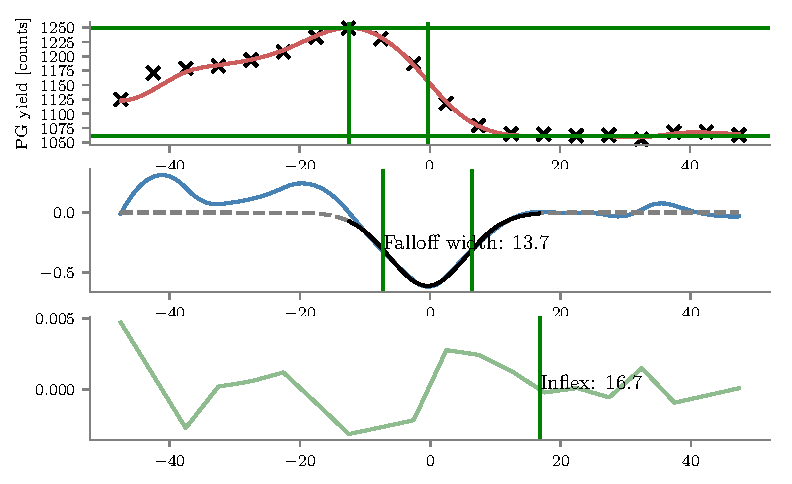
\includegraphics[width=.45\textwidth]{FOW_PMMA_phantom-iba-auger-tof-3}}\quad
  \subfloat[MPS]{\label{FOWMPS}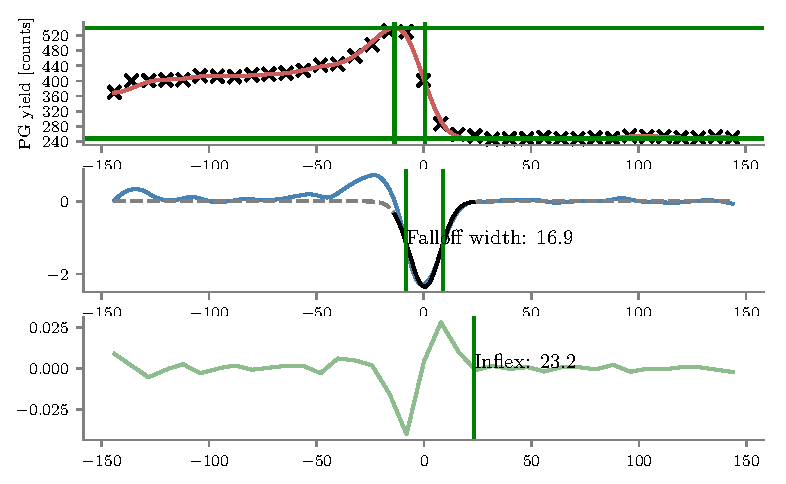
\includegraphics[width=.45\textwidth]{FOW_PMMA_phantom-ipnl-auger-tof-3}}
  \caption{\label{FOWCOMP} MPS and KES FOW estimation illustrated.}
\end{figure}

\textcolor{red}{TODO}

% %%%%%%%%%%%%%%%%%%%%%%%%%%%%%%%%%%%%%%%%%%%%%%%%%%%%%%%%%%%%%%%%%%%%%%%%%%%%%%%%
% \subsection{Spot grouping}

% In particle therapy and particle therapy imaging literature often it is mentioned that a spread out Bragg Peak (SOBP) is achieved by giving the most distal iso-energy layer the highest weight and each successive iso-energy layer is of lower energy and of lower weight. This is correct when positions in the transverse plane (to the beam direction) are considered, for homogeneous phantoms, and when interpolation is not required. Interpolation happens when the energy levels of the beam delivery system do not correspond with the distal tumor contour \citep{0031-9155-57-21-N405}, in which case the dose contour is approximated by spreading the distal dose of the nearest two possible energies (see fig.~\ref{fig:planning}).

% \begin{figure}[htp]
%   \centering
%   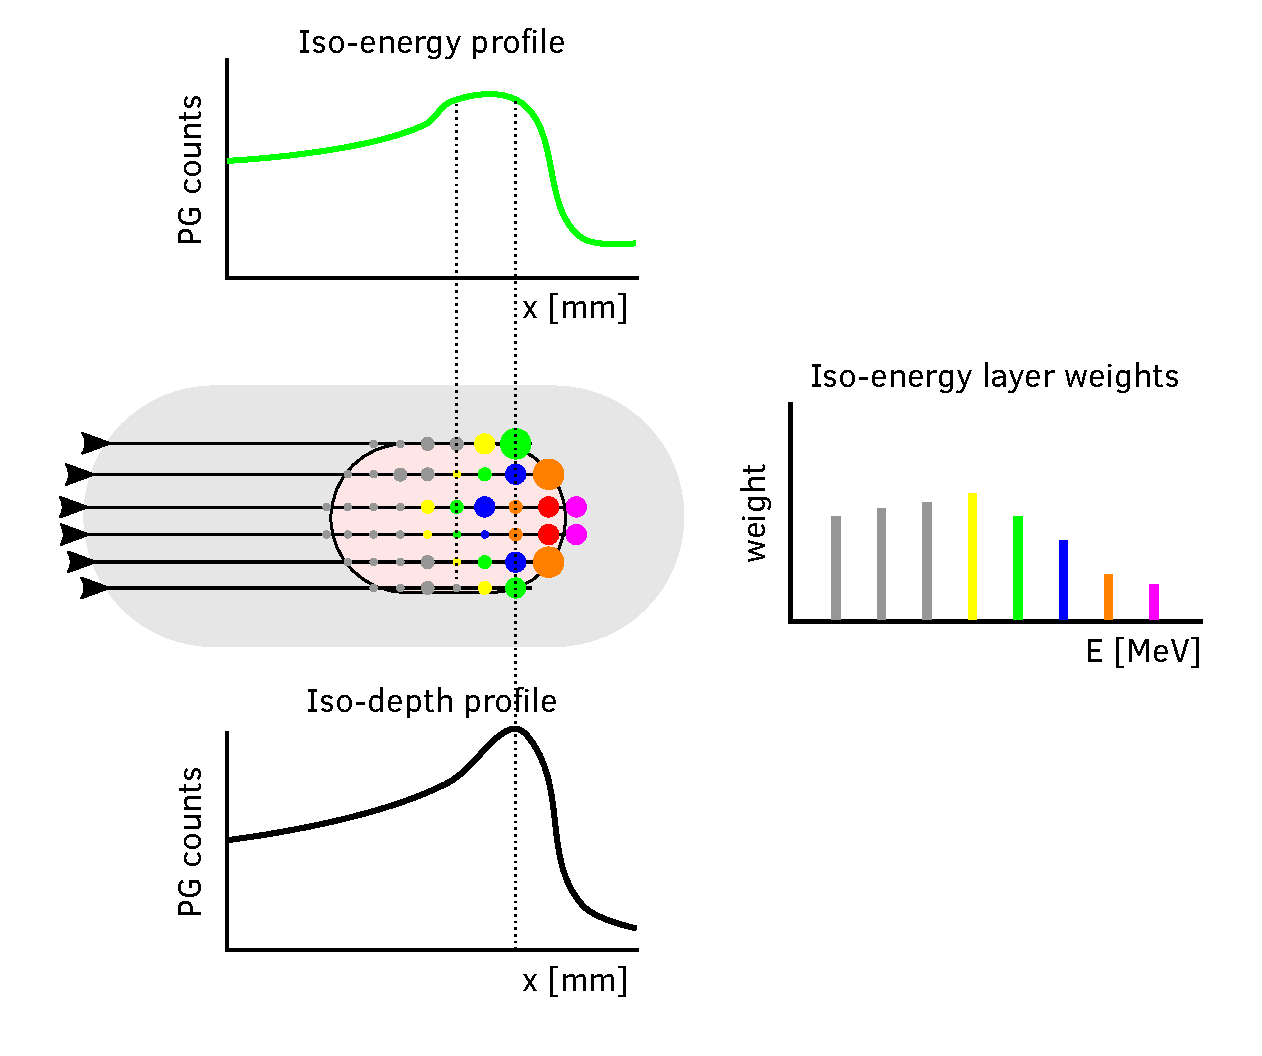
\includegraphics[width=0.6\linewidth]{planning}
%   \caption{A schematic view of a patient (light gray), planned treatment volume (peach-pink), and a proton beam (black horizontal lines coming in from the left). Superimposed are various spots, where the size of the circles indicate spot weights. The spot colors indicate the iso-energy layer of which the spot is part. On the right, the weights (proton counts) per iso-energy layer are plotted, in similar fashion to fig.~\ref{fig:planmid}. On top, the PG profile is sketched for an iso-energy layer. On the bottom, the PG profile is sketched for iso-depth layer (spots of various color on the dotted line). In violet and red, the four dots on the distal end of the two most central beam lines, the effect of interpolation is illustrated: not always is every distal spot planned with a high weight.}
%   \label{fig:planning}
% \end{figure}

% As established in section~\ref{sec:tpanalysis}, a difference was expected between the number of protons per spot as planned and sufficient for reconstruction. Depending on the beam line, the minimum unit of PG detection may be a spot (beam scanning) or an iso-energy layer (passive scattering). Since most new centers employ active beam scanning, new grouping methods are possible. Here a spot grouping method is proposed based on the notion of depth proximity. On the planning CT the 3D dose distribution is computed per spot, and then a dose FOP is determined with the same algorithm as for PG FOP. The FOPs for each spot are binned along the beam line, and these bins we call iso-depth layers. The assumption is that due to inhomogeneities, protons within an iso-energy layer may have very different FOPs in the patient. This iso-depth grouping method will be compared to grouping by iso-energy.


%%%%%%%%%%%%%%%%%%%%%%%%%%%%%%%%%%%%%%%%%%%%%%%%%%%%%%%%%%%%%%%%%%%%%%%%%%%%%%%%
\subsection{Figures of merit}\label{figmerit}

We use the test-case presented in \cite{Perali2014} as the KES detector properties such as background were published for that scenario, again in order to remove any doubt that a difference in camera performance could be due to a difference in implementation or setup. A 160 MeV mono-energetic proton beam is shot into a cylindrical PMMA phantom (length 30 cm, radius 15 cm). Employing the batch method we realize between 50 simulations for each experiment.%, each resulting in a FOP estimate, giving us a mean $\upmu_\textrm{FOP}$ and a standard deviation $\upsigma_\textrm{FOP}$ for a certain experiment. Since we are studying the effect of replacing the CT with a RPCT to simulate patient change, we run each experiment with both CT and RPCT. Each FOP estimate of the N CT realizations is compared to each FOP estimate of the N RPCT realizations, resulting in N$\times$N possible \emph{FOP shift} measurements. These distributions have a $\upmu_\Delta$ and a $\upsigma_\Delta$. The shift initially obtained with the dose is denoted $\Delta_\textrm{dose}$


Grading the performance of the detectors will be done according to these figures of merit: 

%\begin{itemize}[noitemsep]
%\item Accuracy: $| \upmu_{\Delta} - \Delta_\textrm{dose}|$.
%\item Precision: $\upsigma_\Delta$. For this estimate of the standard deviation of the Gaussian distribution a standard deviation can be computed once again based on the number of realization $n$ used to obtain it: $\upsigma(\upsigma_\Delta)=\frac{\upsigma_\Delta}{\sqrt{2\times(n-1)}}$, as per \citet[formula 4.54]{Leo1994}.
%\item Confidence: the percentage of RPCT FOP realizations that fall outside $\upmu_\textrm{FOP,CT}\pm2\upsigma_\textrm{FOP,CT}$ indicates the likelihood any difference from the expected FOP is measured. In other words, given that in this analysis we know that a shift should be detected, what is the probability that a particular realization does so? It will be denoted as P$_\Delta$.
%\end{itemize}

\begin{itemize}
  \item Linear collection efficiency ($LCE$)
  \item[] The LCE is the detection yield in the absorber per unit length of the detector. Since a full MC validation (in particular the background) has not been performed, the most honest way to use the LCE is as ratio between the cameras. Any bias should be divided out.
  \item[] \textcolor{red}{SHOULD we here talk about studying only the MPS/KES ratio? ALSO, will we compare to the formula?}
  \item Spatial resolution ($SR$)
  \item[] The SR is obtained by taking the point spread function of the PG profile in this particular case of the mono-energetic beam in a mono-material box. The BP is as sharp as it can be in such a scenario, and any blur seen in the detected PG profile is then due to the collimator design.
  \item Falloff retrieval precision ($FRP$)
  \item[] The FRP is the standard deviation of the FOP, which is obtained by way of the batch method.
\end{itemize}

Each of these can then be examined as function of the energy and ToF selections.


%%%%%%%%%%%%%%%%%%%%%%%%%%%%%%%%%%%%%%%%%%%%%%%%%%%%%%%%%%%%%%%%%%%%%%%%%%%%%%%%

% \subsection{CT data, treatment plans}

% \begin{figure}[htp]
%   \centering
%   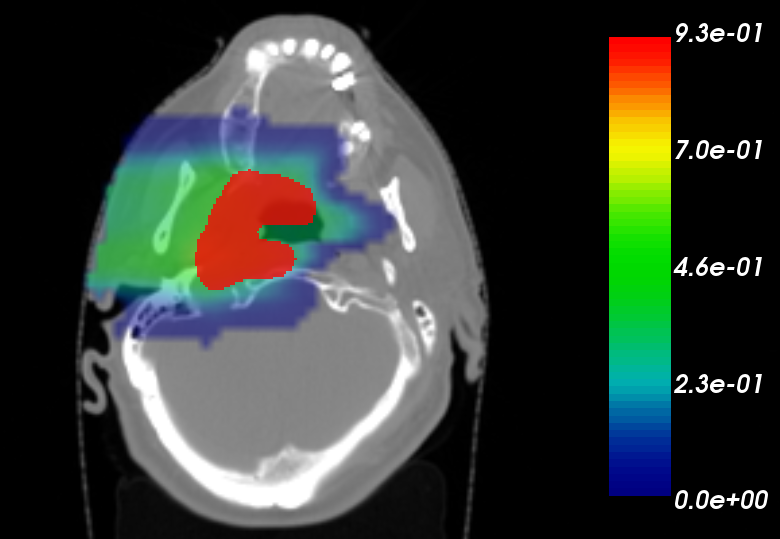
\includegraphics[width=0.5\linewidth]{ourpatient}
%   \caption{A slice of the CT used in this study is shown with the dose due to field 2 of the plan overlaid, color scale in Grey, with in red the planned treatment volume (PTV).}
%   \label{fig:our-patient}
% \end{figure}

% To study real patient change, a planning and replanning CT (CT and RPCT) set was chosen for a patient with a head and neck tumor, wrapped around the trachea. The CT and RPCT were co-registered on bony structures. A realistic two-field TP was created on the CT, and then simulated with Gate \citep{Grevillot2012}. In this paper, only the main field will be studied. The CT with the dose due to this field and the PTV structure are seen in fig.~\ref{fig:our-patient}.

% %%%%%%%%%%%%%%%%%%%%%%%%%%%%%%%%%%%%%%%%%%%%%%%%%%%%%%%%%%%%%%%%%%%%%%%%%%%%%%%%
% \subsection{Spot selection}

% \begin{figure}[htp]
%   \centering
%   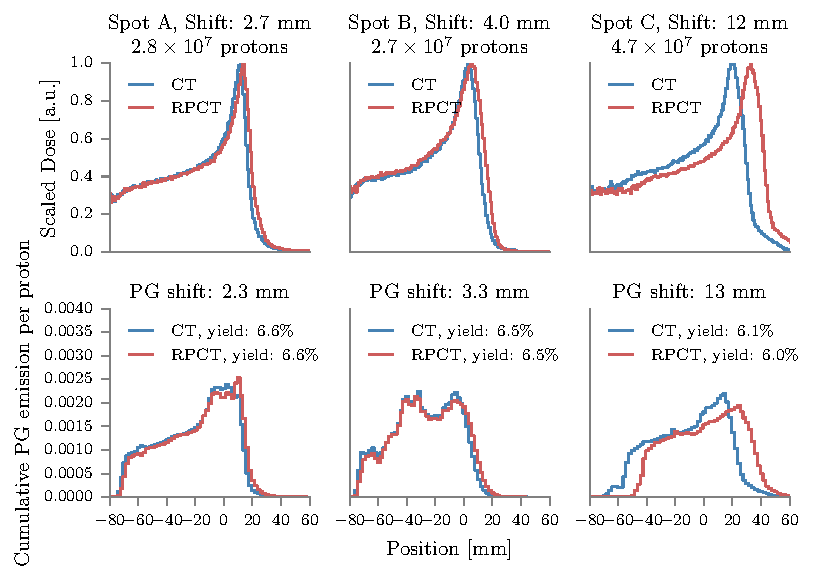
\includegraphics[width=0.99\linewidth]{spotprofiles}
%   \caption{The three chosen spots, based on their shifts and quality of shift. Dose is normalized by mass, which explains the lack of structure. Top row: dose profiles, bottom row: PG emission profiles as used in the second stage of the simulation (PG detection). The yield is the integral yield of the whole image, so 6\% means 6 out of 100 protons generate a PG.}
%   \label{fig:the-spots}
% \end{figure}

% \begin{table}
% \centering
% \begin{tabular}{llll}
% 	 & Spot A & Spot B & Spot C\\
% 	\midrule
% 	Dose shift [mm] & 2.77 & 4.08 & 12.4\\
% 	PG emission shift [mm] & 2.32 & 3.34 & 13.9\\
% 	\midrule
% 	Iso-energy layer [MeV] & 145.86 & 143.02 & 143.02 \\
% 	x-pos [mm] & -24.0 &  -24.0 &  -24.0 \\
% 	y-pos [mm] & 16.0 & 40.0 & -40.0 \\
% 	Nr. protons & $2.75\cdot10^7$ & $2.72\cdot10^7$ & $4.73\cdot10^7$ \\
% \end{tabular}
% \caption{Summary of the properties of the selected spots.}
% \label{table:spotselec}
% \end{table}

% Three spots (table~\ref{table:spotselec}) were selected for presentation in this study. Spot C, with a large shift of over a centimeter with a whiff of overshoot: the beam partially exits the patient causing the distal elevation seen in figure~\ref{fig:the-spots}. An expected shift of over a centimeter should be reliably detectable for any PG camera. Spots A and B are more challenging; with expected shifts between 2 and 4 mm they represent a minimum shift that the PG cameras should be able to detect.



%%%%%%%%%%%%%%%%%%%%%%%%%%%%%%%%%%%%%%%%%%%%%%%%%%%%%%%%%%%%%%%%%%%%%%%%%%%%%%%%


\section{Results}

\subsection{Geometrical considerations}

\subsubsection{Linear collection efficiency}
\textcolor{red}{TODO} detection yields. compare to prediction.
\subsubsection{Spatial resolution}
\textcolor{red}{TODO}
\subsubsection{Falloff retrieval precision}

\begin{table}
\centering
\begin{tabular}{lllllllll}
	\midrule
	Time selection 					& ToF &     &     &     & none&     &     &     \\
	Energy selection 				& 1   &     & 3   &     & 1   &     & 3   &     \\
	Camera 							& MPS & KES & MPS & KES & MPS & KES & MPS & KES \\
	\midrule
 	FOW                         	& 19.7& 20.9& 18.3& 19.3& 19.8& 21.9& 17.9& 23.6\\
 	FOW (perfect collimator) 	& 17.8& 13.7& 16.9& 13.7& 18.3& 14.2& 17.0& 11.6\\
	\midrule
\end{tabular}
\caption{FOW PSF.}
\label{FOWCOMP}
\end{table}

The FOW shown in table~\ref{FOWCOMP} shows that both cameras perform similar with ToF selection. For the MPS the ToF selection makes no difference (up to 2\%), while for the KES it gives a 10-20\% improvement. The results are a bit worse than the calculated values in table~\ref{GeomFormulas}, but close to the 20 mm as postulated in \cite{Priegnitz2015}.

When we make the collimator perfectly absorbing (we kill any tracks entering the material), we can see the KES's effective slit width in action: the transmission through the collimator creating a wider $s_e$ is gone and we see the FOW decrease between 40 and 100\%. This is roughly in line with the calculated $s_e$: \textcolor{red}{ETIENNE?} Surprisingly the FOW of the KES approaches the theoretical value nearly, while the MPS is still a few millimeters worse than calculated.





===================================================

\begin{itemize}
  \item Formulas of the the MPS and KES detection efficiencies and spatial resolution from geometrical considerations (figure~\ref{GeomFormulas})

  \begin{itemize}
    \item Draw some conclusions about the intrinsic features of MPS and KES collimators knowing that the falloff retrieval precision (FRP)   
    \begin{itemize}
      \item Efficiency: same efficiency with the same $s, L, H$, $d_2(\text{KES}) = D(\text{MPS})$, $d_2(\text{MPS})=0$ (no space between collimator and absorber in MPS) and $f\longrightarrow0$ (perfect collimator). In practice, $f\ne 0$ ($f=0.4$ in the CLaRyS MPS camera) so that the KES camera has a slightly larger efficiency than the MPS camera with the aforementioned geometrical conditions. It is worth noting that the KES detection efficiency is not constant over the FOV.
      \item Spatial resolution: same resolution with the same geometrical conditions and perfect collimators. In practice, MPS transparency can be neglected in the CLaRyS prototype ($D = 180$~mm) but not the KES transparency so that the KES camera has a slightly poorer spatial resolution than the one of the MPS camera (still with the aforementioned geometrical conditions).
    \end{itemize}       
    \item Estimate the MPS and KES performances in Smeets 2016 and Lin 2017: the KES/MPS detection efficiency ratio is 1.6 for Smeets 2016 and 5.3 for Lin 2017 (assuming the use of the same energy window) $\Rightarrow$ these comparisons were unfair\dots   
  \end{itemize}
\end{itemize}

\begin{figure}[htp]
  \centering
  \subfloat[Smeets 2016 setup]{\label{SmeetsComparison}
\includegraphics[width=.45\textwidth]{Smeets2016}}\quad
  \subfloat[Lin's setup]{\label{LinComparison}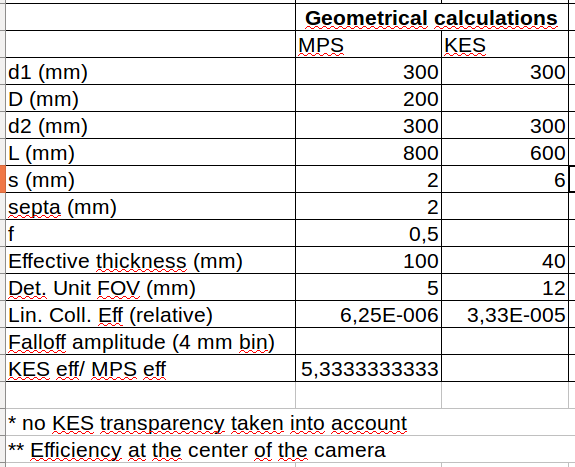
\includegraphics[width=.45\textwidth]{LinComparison}}
  \caption{\label{LitteratureComp} MPS and KES comparisons in litterature.}
\end{figure}   

( \cite{Roellinghoff2014a} shows impact of TOF )

\subsection{Monte Carlo simulations}

\textcolor{red}{TODO: Estimate of the falloff width from the PG profile derivative (see Material and methods section).}

\subsubsection{Geometrical considerations verification}

\textcolor{red}{I think it would be better to show PG profiles with 1-8 MeV energy selection with no TOF selection. The advantage of these selections is that it allows us to show the impact of energy (>1 MeV vs 3-6 MeV selection for KES) and TOF selection (for MPS) when we move to the prototypes configurations. We can put in the table of Figure~\ref{CameraPerformancesFairComp} the result with the 3-6 MeV energy selection to show that the results do not depend on energy selection).}

Figures~\ref{PGprofileFairComp} and \ref{CameraPerformancesFairComp}.

\begin{figure}[!htp]
  \centering
  \subfloat[MPS]{\label{SmeetsComparison}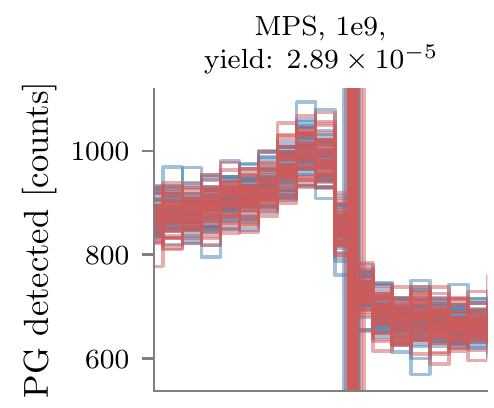
\includegraphics[width=.45\textwidth]{MPS_3-6MeV_noTOF}}\quad
  \subfloat[KES]{\label{LinComparison}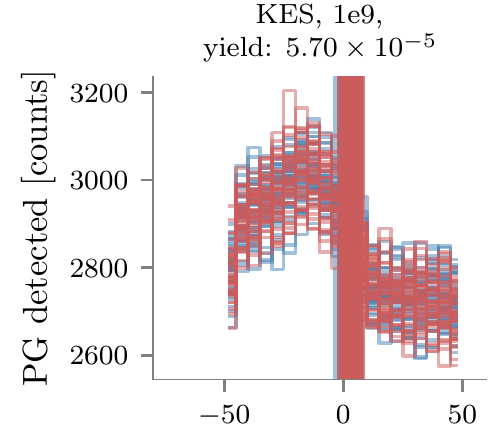
\includegraphics[width=.45\textwidth]{KES_3-6MeV_noTOF}}
  \caption{\label{PGprofileFairComp} MPS and KES comparisons with the same absorber and the same energy (3-6~MeV) and TOF selection (no TOF selection). \textcolor{red}{Sum the statistics of the various 1e9 PG profiles to get the smoothest profiles (we are interested in PG profile shapes). This will allow us to better estimate the falloff features, namely amplitude and width. Put the 2 PG profiles on a single figure?}}
\end{figure}  

\begin{figure}[htp]
  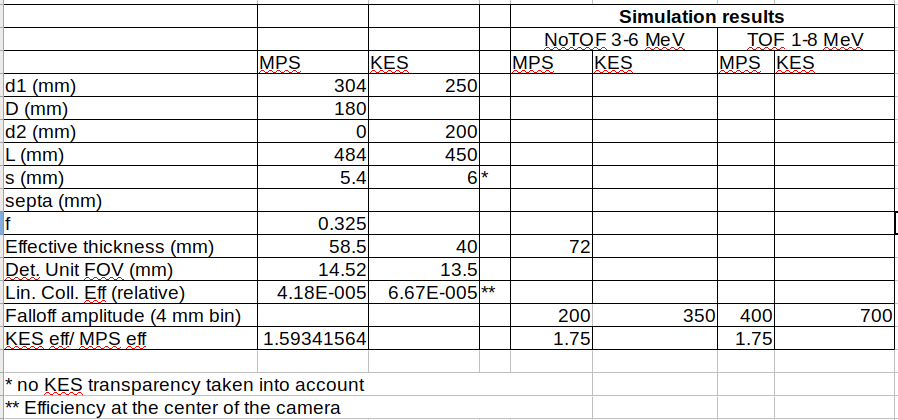
\includegraphics[width=\textwidth]{FairComparison}
  \caption{\label{CameraPerformancesFairComp} MPS and KES comparisons with the same absorber, energy and TOF selection. The first columns of the table correspond to the geometrical calculations. \textcolor{red}{It is interesting to show the results for the two energy selections but it would be nice to have only one TOF selection (no TOF).}}
\end{figure}

\subsection{Clinical case study}

Performance under clinical conditions is the eventual purpose of these PG cameras, and therefore we here include the results of the clinical case study.. Since both cameras prototypes were optimized assuming their particular choice for absorber and energy selection window, here we chose to set 

\paragraph{PG profiles}

Figure~\ref{PGprofileProtoComp}.

\begin{figure}[!htp]
  \centering
  \subfloat[MPS]{\label{SmeetsComparison}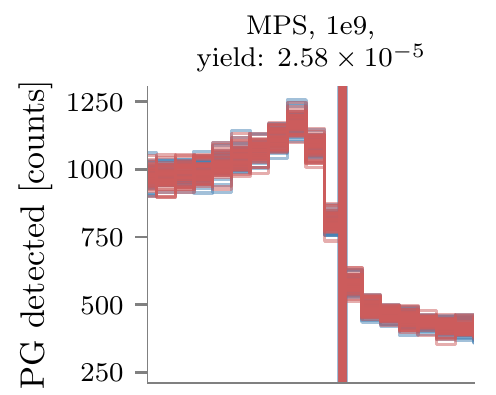
\includegraphics[width=.45\textwidth]{MPS_1-8MeV_TOF}}\quad
  \subfloat[KES]{\label{LinComparison}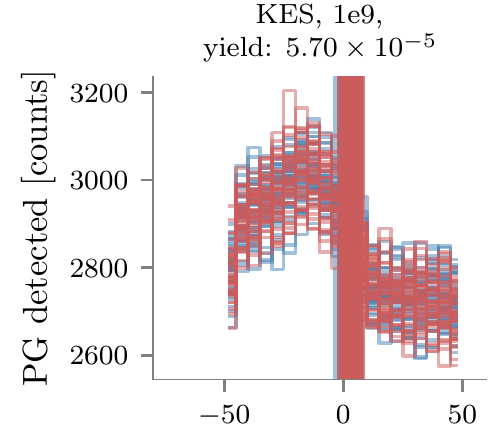
\includegraphics[width=.45\textwidth]{KES_3-6MeV_noTOF}}
  \caption{\label{PGprofileProtoComp} MPS and KES prototypes comparisons. MPS BGO aborber with 1-8 MeV energy selection and TOF selection. KES: LYSO absorber with 3-6 MeV and no TOF selection). \textcolor{red}{Sum the statistics of the various 1e9 PG profiles to get the smoothest profiles (we are interested in PG profile shapes). This will allow us to better estimate the falloff features, namely amplitude and width. Put the 2 PG profiles on a single figure?}}
\end{figure}  

KES/MPS ratio $\sim 400/350 \sim 0.9$.

\paragraph{FRP}

Figure showing the falloff retrieval precision (FRP) (standard deviation of the falloff position distributions) for the 2 prototypes as a function of the number of incident protons ($10^7$, $10^8$, $10^9$).

\textcolor{red}{We do not have this figure yet. The figure in the spot grouping paper shows the mean and standard deviations on the falloff position differences for the 3 spots considered. }

%%%%%%%%%%%%%%%%%%%%%%%%%%%%%%%%%%%%%%%%%%%%%%%%%%%%%%%%%%%%%%%%%%%%%%%%%%%%%%%%
\section{Discussion}


%%%%%%%%%%%%%%%%%%%%%%%%%%%%%%%%%%%%%%%%%%%%%%%%%%%%%%%%%%%%%%%%%%%%%%%%%%%%%%%%
\section{Conclusion}


%%%%%%%%%%%%%%%%%%%%%%%%%%%%%%%%%%%%%%%%%%%%%%%%%%%%%%%%%%%%%%%%%%%%%%%%%%%%%%%%
\section{Acknowledgements}

This work was partly supported by SIRIC LYric Grant INCa-DGOS-4664, LABEX PRIMES (ANR-11-LABX-0063 / ANR-11-IDEX-0007) and Fondation ARC. The authors would like to thank Marie-Claude Biston, Thomas Baudier and Gloria Vilches-Freixas for their help finding the CT images and making the treatment plan. We also thank Erik Almhagen and Uppsala University Hospital, Sweden for the treatment plan data presented in this paper.

%%%%%%%%%%%%%%%%%%%%%%%%%%%%%%%%%%%%%%%%%%%%%%%%%%%%%%%%%%%%%%%%%%%%%%%%%%%%%%%%
\newpage

\appendix
% \begin{appendices}
% 
%%%%%%%%%%%%%%%%%%%%%%%%%%%%%%%%%%%%%%%%%%%%%%%%%%%%%%%%%%%%%%%%%%%%%%%%%%%%%%%%

\section{Fall-off position estimation procedure}\label{sec:fopproc}

\begin{enumerate}[noitemsep]
\item The measured PG profile is smoothed and interpolated with a smoothing spline function:

\begin{equation}
\sum_{i=1}^n (y_i - \hat f(x_i))^2 + \lambda \int_{x_1}^{x_n} \hat f''(x)^2 \,dx
\end{equation}

where $y_i$ is the measured PG profile and $x_i$ the associated x-coordinates, $\hat f(x_i)$ the estimate smoothed spline function and $\lambda$ a smoothing parameter that determines the penalty for deviating from measurement in exchange for smoothness (second order derivatives are close to zero on smooth functions). $\lambda = 0$ produces a perfect spline fit to the data, while $\lambda \gg 1$ produces a horizontal line. We found that $\lambda = 2$ provided an acceptable trade-off between overfitting to noise and removing too many features, which tends to happen for low statistic measurements.
\item The obtained function is plotted for 1024 $x_j$, an number that provided a sufficiently high resolution. Any $f(x_j) < 0$ are set to $0$. 
\item The global maximum is found.
\item The baseline is set equal to the lowest 25\% of bins.
\item From the distal end backwards, the first maximum is taken as the distal most peak position, if it is above the threshold of 30\% of the difference between baseline and global maximum. If no such point is found, the global maximum is taken as the distal most maximum.
\item The fall-off amplitude (FOA) is set to the difference between the distal maximum and baseline: $FOA = max-baseline$. The FOP is obtained by traversing the smoothed profile from the distal end towards the peak until $y_j > \frac{1}{2}FOA$.
\end{enumerate}

The results of this procedure are illustrated in figure~\ref{fig:our-fit}. Every PG profile was estimated 50 times, and so we obtained 50 estimates for the FOP. It is assumed that the FOPs follow a Gaussian distribution, so the mean of the 50 realizations gives the best FOP estimate and the sigma gives the precision of the ability to estimate the best FOP. Comparing the 50 FOP estimates obtained from the CT with the 50 estimates obtained from the RPCT simulations, gives 2500 possible shift estimates. Again, the distribution of shifts should be centered at the true shift, while the sigma indicates how likely it is that this true shift is detected under the current conditions.

\begin{figure}[htp]
  \centering
  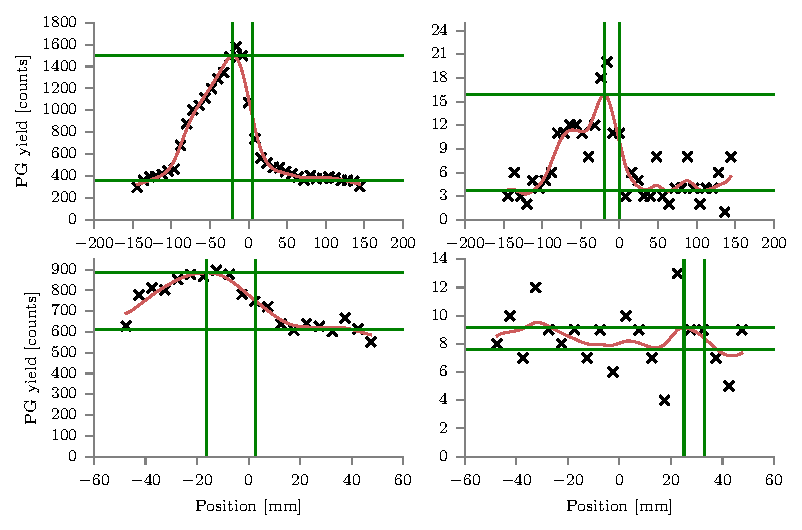
\includegraphics[width=0.9\linewidth]{fopproc}
  \caption{The top row demonstrates the fall-off determination procedure on the multi-parallel camera data; on the bottom row on knife-edge slit camera data. The left column is produced with a PG signal due to $10^9$ primaries, while the right column was produced with $10^7$ primary protons. In black crosses the measured PG counts are plotted. The smoothed data is shown in red. The green horizontal lines are drawn at the obtained distal maxima and baselines, while the vertical green lines shown the position of the distal maximum and the position of the fall-off. For the bottom-right plot, a history is visible where the procedure fails: the background induces an erroneous peak detection.}
  \label{fig:our-fit}
\end{figure}

\section{Verification of the cameras}

In \cite{Priegnitz2015} PG shifts due to beam energy shifts are studied for the KES camera: the \emph{detectability} of the fall-off as function of the number of primaries. Here that simulation was recreated: a mono-energetic beam shoots into a waterbox at two energies. 50 realizations are generated with a 139 MeV beam energy, and 50 realizations with 144 MeV. At $10^9$ primaries, the distributions are well separated with a shift of 8.3 mm (different from \cite{Priegnitz2015} because of the different material). In figure 13 in \cite{Perali2014} with $10^9$ primaries a standard deviation of 1.5 mm is obtained, while here 1.21 and 1.14 mm were obtained. It is sufficient agreement to be confident of our setup and further results.

The KES prototype's sensitivity to accurate positioning with respect to the expected FOP was elaborated upon in \citet[Section IV.A.3]{Sterpin2015}: the detector response is, due to the KES collimator, not linear as with a parallel slit collimator. In this study, to make the comparison as fair as possible and avoid any bias, alignment on the FOP specific for each spot was ensured as follows: the intermediate PG source image of vpgTLE (equivalent to the PG emission) was projected on the beam axis, and then convolved with a Gaussian of $\upsigma = 8.5$ mm, which corresponds to the point spread function (PSF) with a FWHM of 20 mm used in \cite{Priegnitz2015} to approximate the detected profiles from the emitted profile. These profiles will be referred to as "PG + PSF" profiles. As a matter of fact, the MPS prototype has roughly the same PSF as the KES prototype so that "PG + PSF" fall-off position can be considered as the expected position for both cameras.

To verify the implementation of the MPS camera, the precision on the FOP, obtained with the procedure outlined in the previous paragraph, is compared to earlier results. In the caption of figure 9 in \cite{Pinto2014a} it is stated that with $10^8$ primaries a standard deviation of 1.3 mm is obtained for the detector design used here, which is about 20\% different from the results obtained in this study: 1.63 and 1.54 mm.
%%%%%%%%%%%%%%%%%%%%%%%%%%%%%%%%%%%%%%%%%%%%%%%%%%%%%%%%%%%%%%%%%%%%%%%%%%%%%%%%
% \end{appendices}
\newpage

%%%%%%%%%%%%%%%%%%%%%%%%%%%%%%%%%%%%%%%%%%%%%%%%%%%%%%%%%%%%%%%%%%%%%%%%%%%%%%%%

\bibliographystyle{plainnat}
\bibliography{lib.bib}
\end{document}%\grid
